%https://tex.stackexchange.com/questions/584590/tikz-double-sideband-dsb-spectrum
\documentclass[tikz,border=3.14159mm,subpreambles=true]{standalone}

\providecommand{\DSBA}[5]{
    \def\xa{#2} \def\ya{0}
    \def\xb{\xa/2} \def\yb{#5}
    \def\xc{0} \def\yc{#5}
    \def\tang{\xa/3}
    %   
    \def\curve{
            (#1-\xa,\ya) .. controls ++ (2*\tang,0) and ++ (-\tang,0) ..
            (#1-\xb,\yb) .. controls ++ (.5*\tang,0) and ++ (-\tang,0) ..
            (#1,\yc) .. controls ++ (\tang,0) and ++ (-.5*\tang,0) ..
            (#1+\xb,\yb) .. controls ++ (\tang,0) and ++ (-2*\tang,0) ..
            (#1+\xa,\ya)
            }
    \path[fill=#3!#4] (#1-\xa,0) -- \curve -- (#1+\xa,0) -- cycle;
    \draw  \curve;
    }
\providecommand{\DSBB}[5]{
    \def\xa{#2} \def\ya{0}
    \def\xb{\xa/2} \def\yb{#5}
    \def\xc{0} \def\yc{#5}
    \def\tang{\xa/3}
    %   
    \def\curve{
            (#1-\xa,\ya) .. controls ++ (2*\tang,0) and ++ (-\tang,0) ..
            (#1-\xb,\yb) .. controls ++ (.5*\tang,0) and ++ (-\tang,0) ..
            (#1,\yc) .. controls ++ (\tang,0) and ++ (-.5*\tang,0) ..
            (#1+\xb,\yb) .. controls ++ (\tang,0) and ++ (-2*\tang,0) ..
            (#1+\xa,\ya)
            }
    \path[fill=#3!#4,opacity=0.6] (#1-\xa,0) -- \curve -- (#1+\xa,0) -- cycle;
    \draw[color=#3!#4,opacity=0.8]  \curve;
    }
\providecommand{\DSBC}[5]{
    \def\xa{#2} \def\ya{0}
    \def\xb{\xa/8} \def\yb{#5}
    \def\xc{0} \def\yc{#5}
    \def\tang{\xa/5}
    %   
    \def\curve{
            (#1-\xa,\ya) .. controls ++ (2*\tang,0) and ++ (-\tang,0) ..
            (#1-\xb,\yb) .. controls ++ (.5*\tang,0) and ++ (-\tang,0) ..
            (#1,\yc) .. controls ++ (\tang,0) and ++ (-.5*\tang,0) ..
            (#1+\xb,\yb) .. controls ++ (\tang,0) and ++ (-2*\tang,0) ..
            (#1+\xa,\ya)
            }
    \path[fill=#3!#4,opacity=0.6] (#1-\xa,0) -- \curve -- (#1+\xa,0) -- cycle;
    \draw[color=#3!#4,opacity=0.8]  \curve;
    }


        
\begin{document}
    
    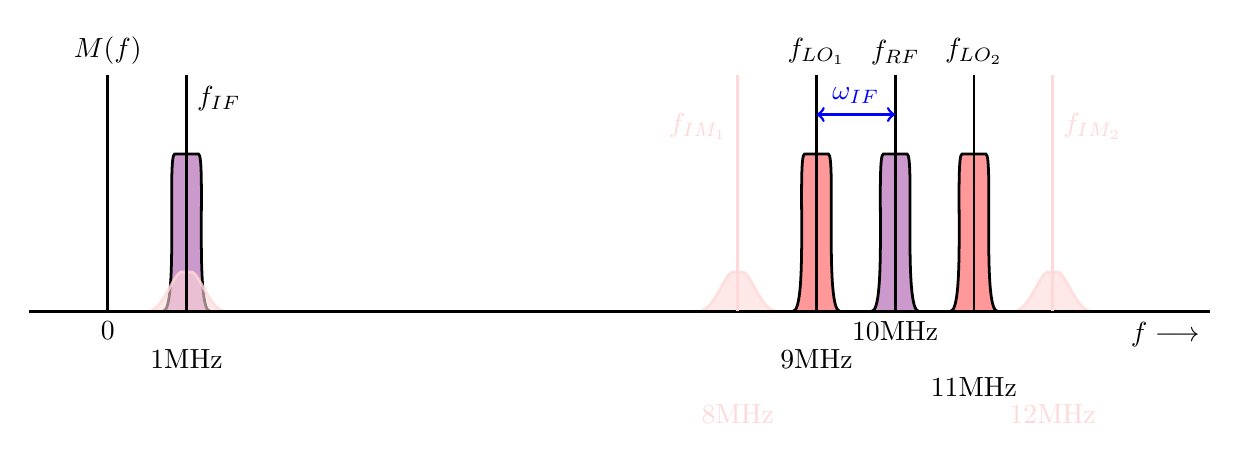
\begin{tikzpicture}[
        line width=1pt,
        sb/.style={text width=1.5cm, align=center,inner sep=0pt}]
        
    \DSBA{10}{0.3}{violet}{40}{2}
    \DSBA{9}{0.3}{red}{40}{2}
    \DSBA{11}{0.3}{red}{40}{2}
    \DSBA{1}{0.3}{violet}{40}{2}
    \DSBC{8}{0.5}{pink}{60}{0.5}
    \DSBC{12}{0.5}{pink}{60}{0.5}
    \DSBC{1}{0.5}{pink}{60}{0.5}
    \draw   (-1,0) -- (14,0) node [below left] {$f \longrightarrow$}
            (0,0) node[below] {0} --++ (0,3) node [above] {$M(f)$}
            (10,0) node[below] {10MHz} --++ (0,3) node [above] {$f_{RF}$}
            (9,0) node[below,yshift=-10] {9MHz} --++ (0,3) node [above ] {$f_{LO_{1}}$}
            (11,0) node[below,yshift=-20] {11MHz} --++ (0,3) node [above ] {$f_{LO_{2}}$}
            (1,0) node[below,yshift=-10] {1MHz} --++ (0,3) node [below right] {$f_{IF}$};
    \draw[<->, color=blue] (9,2.5)--(10,2.5);
    \node[align=center, above, color=blue] at (9.5,2.5) {$\omega_{IF}$};
    \draw[color=pink!60] (8,0) node[below,yshift=-30,color=pink!60] {8MHz} --++ (0,3) node [below left,yshift=-10,color=pink!60] {$f_{IM_{1}}$}
    (12,0) node[below,yshift=-30,color=pink!60] {12MHz} --++ (0,3) node [below right,yshift=-10,color=pink!60] {$f_{IM_{2}}$};
    
                
    \end{tikzpicture}
\end{document}